\documentclass[10pt, conference]{IEEEtran}
% The preceding line is only needed to identify funding in the first footnote. If that is unneeded, please comment it out.
\usepackage{cite}
\usepackage{amsmath,amssymb,amsfonts}
\usepackage{graphicx}
\usepackage{textcomp}
\def\BibTeX{{\rm B\kern-.05em{\sc i\kern-.025em b}\kern-.08em
    T\kern-.1667em\lower.7ex\hbox{E}\kern-.125emX}}
\begin{document}

\title{Midterm Report\\
}

\author{\IEEEauthorblockN{Travis Bartley}
}

\maketitle

\begin{abstract}
This paper provides an empirical demonstration of the optimality of discrete Bayes classifiers by measuring expected gain over idealized data sets. Uniformly random distributions of class-measure pairs are generated from a five-dimensional measurement space and  fitted through iterative biasing towards improving classifier performance. This fitting is repeated over variations in class ranges and sampling sizes to examine the relationship between requisite variety and classifier performance. Classifier performance is considered generally invariant over all variations, with a slight trend to under-perform with an increasing range of class values.   
\end{abstract}

\section{Introduction}
	Bayesian classification is a common methodology in which maximum \textit{a posteriori} estimation is utilized for the creation of decision rules for classification tasks. Along with being trained in linear time \cite{b1} and conceptually intuitive, they hold prominence for their demonstrable property of optimality when utilized in tasks evaluated on metrics of expected value.  Indeed, by definition the decision rule produced through Bayesian classification is the function that defines the upper bounds of expected value for a decision task, exceeding the cost-gain estimation of any other classifier. That is, for any Bayesian decision rule $f$:
\begin{equation}
E[e; f] \geq E[e;g]
\end{equation}
where $E$ is the expected gain estimation function, $g$ is any arbitrary decision rule, and $e$ is the economic cost matrix for the assignment of a class value to a measurement given the measurement's true class value.   

However, the conceptual simplicity and ease of calculation that merit the classifier$'$s use can also be disadvantageous. Given a set of measurement values, the classifier function chooses the class assignment that maximizes the sum of all possible economic gain  values for all possible true class assignments, weighted by the conditional probability of each true assignment given the measurement being classified. Such may be expressed as the function that assigns $c^k$ to measurement tuple $d$ when
\begin{equation}\label{eq:expectedGain}
\sum_{c^j \in C}{e(c^j, c^k)P_T(c^j|d)} \geq \sum_{c^j \in C}{e(c^j,c^n)P_T(c^j|d)} 
\end{equation}
where $C$ is the set of all class values,  $d$ is a member of measurement space $M$, $P_T(c|d)$ is the probability of class $c$ being the true classification of $d$ given $d$ in the measurement set, and $e_{i,j}$  the economic cost of $e$ for the assignment of a measure to class $j$ when it was of real class $i$.  For derivation of $P_T(c|d)$, Bayes$'$ theorem is used:
\begin{equation}
P_T(c|d)=P(d|c)P(c)/P(d)
\end{equation}
or, as $P(d)$ is typically canceled out in the derivation of expected gain, it may be expressed with solely the numerator:
\begin{equation}\label{eq:BayesNumerator}
P(d|c)P(c)
\end{equation}
While the calculation of $P(c)$ can be reliably estimated from a suitably robust measurement set of size proportionate to $K = |C|$, the observation of all possible measurement-class pairs for derivation of $P(d|c)$ requires a set-size proportionate to $K\cdot S$. For low probability pairs, this question of sample size becomes more pertinent, as a failure to witness a pair in a training set poses the issue of assigning a zero value to a non-zero $P_T(c|d)$ \cite{b1}, limiting classifier accuracy. While this issue may be ignored for relatively simple classification tasks, orientation towards real-world applications poses a demand for sample sizes that are infeasible for many tasks (e.g. sentiment analysis of natural language) \cite{b2}. 

To address the likely poverty of training data, numerous methodologies are typically employed. Accommodating the simple necessity of non-zero probabilities,  one may add a ‘smoothing’ factor $\Delta$ to all conditional probability entries and normalize the distribution for each class \cite{b4}. Such allows for calculation of \textit{a posteriori} distributions that observe measurement-value pairs that may have not been present in the training, though at the cost of skewing real distributions and removing any authentic zero probabilities from the data. Subspace classifier projection permits reduction of nonessential measurement features, reducing the measurement space and thus the minimum threshold for possible data accuracy. Given suitable knowledge of the measurement space, the conditional priors may also be approximated through a known probability distribution (e.g. Gaussian distribution for parametric variables, Bernoulli distribution for binomial measures). As well, assuming independence among features, a $'$naive$'$ Bayes estimation of conditional values may also be used \cite{b1} \cite{b2}, calculating the \textit{a posteriori} of a set of measurements as a product of the independent conditional distribution of a measurement's features. That is, for measurement $d$ possessing $n$ measurements $(x_1,x_2,....,x_n)$,
\begin{equation}
P_t(c|d) = P(x_1,...x_N|c)=\prod_{n=1}^N p(x_n|c)
\end{equation}
 Such reduces the need for training data to exhibit all measure-class pairs and instead simply need to be robust enough for observing all values for the individual features. As such, the minimum observation size would be proportionate to $K \cdot R$, with R being the cardinality of the largest feature space. 

Core to the above is the trade-off of providing approximations of the \textit{a posteriori} distributions instead of their true derivations. While such approximations seem to have marginal effects on the "surprising" performance  of Bayesian classifiers \cite{b1}, they do nonetheless leave open the theoretical concern of lacking opportunities to observe exclusive performance of the classifier, particularly in the case of empirically validating ideal testing sets for performance or observing rates of aymptotic error (a feature claimed by Ng and Jordan) \cite{b3}. 

To address this, this paper will present experimental findings of Bayesian classification of synthetic data sets specifically generated for ideal performance. Classifiers are constructed for a randomly generated five-dimensional measurement space, varying in size of sample set and range of possible classes for classification. After establishing a baseline performance for the classifier, the probability distributions used for generating the measurement space and classifier are updated to improve performance. With ideal measurement spaces provided for each classifier, performance is once again evaluated and compared across classifier groups. From this evaluation, it is demonstrated that discrete Bayesian classifiers are largely invariant to variation in measure sizes and only slightly disadvantaged by the increase of class range size, validating their use for supervised learning tasks.
\section{Technical}
\subsection{The classifier}
As detailed in (1-5) above, a Bayesian calssifier is the function that assigns measurement $d$ class $c_k$ fullfilling the expected gain equation:
\begin{equation*}
\sum_{c^j \in C}{e(c^j, c^k)P_T(c^j|d)} \geq \sum_{c^j \in C}{e(c^j,c^n)P_T(c^j|d)}
\end{equation*}
where $P(c|d)$ is derived from the equation:
 \begin{equation*}
P_T(c|d) \propto P(d|c)P(c)
\end{equation*}
 As such, the classifier requires three features: the distribution of class probabilities $P(c)$, the distribution of class-conditional probabilities $P(c|d)$, and an economic gain matrix of $K$x$K$, where each entry $e_{ij}$ refers to the economic gain/cost for assigning class  $j$ to a measure of real value $i$. 
	
	For initializing the classifier, a matrix of class conditional values was generated as follows: given the set of classes $C$, cardinality $K=|C|$, measurement space $M= \{d_1,d_2,....,d_L\}$ where $d_l = (x_1,x_2,....,x_N)$ and cardinality $S=|M|$,  $K$ arrays of length $S$ were generated. For each value of each array, a uniform number was generated between $[0,1]$. After each array $A_c$ was filled, all values were normalized so $\sum_{i=1}^{S}a_i=1$, with $a_i$ being the $i$th element of $A_c$. These $K$ matrices were then treated as tables of class conditional probability values, with $P(c_i|d_j)$ being expressed by the $j$th element in array $A_i$. 
	
	Prior probabilities were generated from the training set, calculating the proportion of each class $c_k'$s occurrence within a given training set. Meanwhile, economic gain matrices were generated as detailed in the following section.
\subsection{The economic gain matrix}
	Prior to testing, two economic $K \times K$ gain matrices are generated for a classifier. The first is the identity matrix, a collection of values that assign zero to any incorrect classification and 1 to a correct classification. One notes that the identity matrix alters the classifier function to one maximizing a measure$'$s conditional \textit{a posteriori}, as:
\begin{equation*}
\sum_{c^j \in C}{e(c^j, c^k)P_T(c^j|d)} \geq \sum_{c^j \in C}{e(c^j,c^n)P_T(c^j|d)} 
\end{equation*}
\begin{equation*}
1 \cdot P_T(c^k|d) + 0 \cdot (K-1) \geq 1 \cdot P_T(c^n|d) + 0 \cdot (K-1)
\end{equation*}
\begin{equation}
P_T(c^k|d) \geq P_T(c^n|d)
\end{equation}

The other matrix used was a penalty matrix that shared reward values for correct identification but substituted a $-1$ cost for any incorrect classification. Such was chosen for two purposes: the first was allowing evaluation of a punitive metric for evaluation and allow evaluation of differences in philosophies of punitive and reward based classification. The second was for validation of the classifier$'$s performance. By the expected gain calculation:
\begin{equation}
E(e) =  \sum_{i=1}^K \sum_{j=1}^K e(c^i,c^j)P_{TA}(c^i, c^j)
\end{equation}
one notes that the identity matrix produces the sum:
\begin{equation}
E(e_{identity}) =  \sum_{j=1}^K P_{TA}(c^j, c^j)
\end{equation}
as all entries $e(c^i,c^J) i \neq j$ are 0, producing the accuracy metric for the classifier. Meanwhile, the penalty matrix evaluates to:
\begin{equation*}
E(e_{penalty}) =  \sum_{i=1}^K \sum_{j=1}^K e(c^i,c^j)P_{TA}(c^i, c^j) 
\end{equation*}
\begin{equation}
E(e_{penalty}) =  -\sum_{i=1}^K \sum_{j=1}^K P_{TA}(c^i, c^j) , c^i \neq c^j
\end{equation}
which is the negative probability of incorrect classification. That is, is is the negative complement of $E(e_identity)$ such that
\begin{equation}
E(e_{identity}) - E(e_{penalty}) = 1 
\end{equation}
Using both the identity and punitive economic gains thus allows validation of accurate performance of the evaluation metric across randomized trials as their difference should sum to $1$ (ignoring the possibility of floating point error).

For reference, matrix representations of each form are provided as follows:
\begin{equation}
e_{identity} = 
\begin{pmatrix}
1 & 0 & \cdots & 0 \\
0 & 1 & \cdots & 0 \\
\vdots  & \vdots  & \ddots & \vdots  \\
0 & 0 & \cdots & 1 
\end{pmatrix}
\end{equation}
\begin{equation}
e_{penalty} = 
\begin{pmatrix}
0 & -1 & \cdots & -1 \\
-1 & 0  & \cdots & -1 \\
\vdots  & \vdots  & \ddots & \vdots  \\
-1 & -1 & \cdots & 0
\end{pmatrix}
\end{equation}
\subsection{Measurements}
For initial data, measurements were generated at random through a uniform distribution. $S$ values from $[0,1]$ were generated and normalized so for generated values $\{s_1,s_2,....s_S\}, \sum_{i=1}^Ss_i = 1$.  Values were then converted into cumulative probability distribution $\{p_1,p_2,...,p_S\}$ to represent the distribution of all measurements in space $M$. 

A similar procedure was conducted for generating classes for measures. $K$ random samples were taken from a uniform distribution $[0,1].$ These samples $\{k_1,k_2,....,k_K\}$ were normalized so $\sum_{j=1}^Kk_j=1$ and then transformed into a cumulative probability distribution $\{q_1,q_2,....,q_K\}$.  An array of length $S$ was then generated with $S$ samples from the same uniform distribution. For each sample $s$, index $c$ was chosen  so as to fulfill the inequality:
\begin{equation}
q_{c-1} \leq s \leq q_c 
\end{equation}
As the cumulative probability distribution organizes $K$ elements as $\{q_1 \leq q_2 \leq .... \leq q_K\}$, this index maps each $s$ to a class value mimicking the synthetic probability distribution, effectively creating a mapping function $\{h: M -> C\}.$

These distributions provide for random generation of samples that conform to a synthetic probability distributions of $d\in M$ and $c \in C.$ $Z$ samples are taken from the uniform distribution $[0,1]$ and then assigned the value $s$ such that for sample $z$:
\begin{equation}
p_{s-1} \leq z \leq p_s 
\end{equation}
As with class assignment, the cumulative probability distribution permits the use of $d$ as an index for measurement $s_d$ in the array of $S$ values so that $z$ maps to measurement $d$ of $M$. This measurement is then mapped to the corresponding $c$ from the class assignment distribution, providing randomly sampled measurement-value pairs. 
\subsection{Testing Protocol}
\subsubsection{Synthetic Measures}
For each test, $Z$ measure-value pairs are generated from a 5-dimensional space $M.$ Then, $K$ conditional probability distributions of length $S=|M|$ are generated, along with the two $K \times K$ economic gain matrices detailed above. 
\subsubsection{V-fold Testing}
Measurements were then shuffled and partitioned for V-folds evaluation with V-factor 10 (chosen empirically).  The classifier was trained on 9 partitions of the measurements to estimate $P(c)$ and then tests were performed on the 10th partition. This was repeated for each combination of ${10 \choose 9}$.
\subsubsection{Evaluation}
For each round of V-fold testing, a $K \times K$ confusion matrix $Q$ was produced, with $q_{ij}$ representing the counts of class assignment $j$ for real class value $i$. After all rounds of V-fold validation were completed, all matrices were summed and then normalized so $\sum_{i=1}^K \sum_{j=1}^K q_{ij} = 1,$ producing probability values for the assignment of class $j$ to measurements of real class $i$, $P_{TA}(c^i, c^j).$  With the provided economic gain matrix $e$, expected gains were calculated by:
\begin{equation*}
E(e) =  \sum_{i=1}^K \sum_{j=1}^K e(c^i,c^j)P_{TA}(c^i, c^j)
\end{equation*}
providing the evaluation metric for each classification.
\subsubsection{Fitting}
To fit data to improve classifier performance, a two-fold technique was used. After each set of V-fold testing, the distribution of class conditional values $P(d|c)$ were increased by $\Delta=.005$ (value empirically determined) for each measurement-class pair seen in the data. Then, each set of conditional values were normalized so $\sum_{d \in M}P(d|c) =1$ for each class. Doing so, the classifier biased itself towards pairs observed in the data-set while reducing preference for unobserved pairs, better fitting it for the data.

This updated class-conditional distribution was then used to regenerate measurement-class pairs. The probability distribution of measurement $d \in M$ was recalculated as:
\begin{equation}
P(d) =  \sum_{c \in C}P(d|c)P(c). 
\end{equation}
with $P(c)$ generated from the entire set of measures-value pairs first generated and held constant over all rounds of fitting. These measurements were then converted into a cumulative probability distribution and used to generate samples as detailed above.

For class assignment, Bayes$'$ rule was used to calculate $P(c|d)$. For each $d$, a cumulative probability distribution of $P(c|d)$ across all classes $c\in C$ was generated. A random sample was taken from uniform distribution $[0,1]$ and then a class index was calculated by using the same inequality from the generation procedure, providing a new set of class assignments for all $d$. 

With the new probability distributions calculated based off the conditional probability used for the generation of the new classifier, $Z$ measurement-class pairs are generated as before, followed by another iteration of V-fold testing for evaluation. This was performed over 10 iterations for each classifier to achieve a final idealized data set.
\section{Experiments}
\subsection{Measure Space}
For experiments, all evaluation was performed for 5-dimensional measurement space $M,$ with each dimension having 10 potential measurement values (determined empirically for ease of testing), providing  $|M| = 10^5=100000$ measurement values. Each tuple of measurement values $(x_1,x_2,....,x_5)$ was converted to a linear representation $L$ through row conversion formula:
\begin{equation}
L = \sum_{k=1}^d (\prod_{q=k+ 1}^5 N_l ) n_k
\end{equation}
with $n_k$ being the $k$th feature of measure $d$ and $N_k$ being the cardinality of $k$th dimension of $M$. One notes that this conversion of 5 feature tuples to single linear indexes reduces the dimensionality of $M$ to be a question of quantity instead of complexity, allowing no loss of generality of experimental findings for other dimensionalities of $M$.
\subsection{Variants}
To observe the relationship between class complexity, sample size, and choice of economic gain matrix on classifier accuracy, experiments were ran over combinations of the following factors:

- Class ranges: $K = 2,4,6.$

- Sample sizes: $Z= S, SK, 2SK$ 

- Economic Gain Matrix: Identity, Penalty

Class range values were chosen to examine variation as class complexity was increased from a binary classification task. Sample range values were chosen to examine effects of minimum sample sizes for viewing all measurements, $Z=S$ and all measurement-class pairs, $Z= SK$. To provide a more realistic chance of obtaining a representative sample, a larger sample size, $Z = 2SK$ was also examined. 

The fitting factor $\Delta$ was .005, added over 10 iterations. Increase in expected value was charted over each iteration.

Each experiment is produced by a unique seed for repeat evaluation. The seed for each experiment is listed with its resultant set of data. 
\section{Results}
For all tests, the difference of expected gain between the identity and penalty matrices summed to 1(within tolerance of floating point error), verifying performance. As such, values presented will be for experiments conducted on the identity matrix. 
\subsection{Initial Results}
Expected gain values before and after fitting are displayed in Table 1
\begin{table}[htbp]
\caption{Expected Gain Before and After Fitting}
\begin{center}
\begin{tabular}{|c|c|c|}
\hline
\textbf{Classifier Parameters}&\multicolumn{2}{|c|}{\textbf{Expected Gain}} \\
\cline{2-3} 
\textbf{} & \textbf{\textit{Before}}& \textbf{\textit{After}}\\
\hline
$K=2,Z=S,seed=2580$&$0.86318$&$0.99981$\\
\hline
$K=2,Z=KS,seed=2590$&$0.51288$&$0.99990$ \\
\hline
$K=2,Z=2KS,seed=2600$&$0.51840$ & $0.99986$  \\
\hline
$K=4,Z=S,seed=2550$&$0.37808$&$0.99924$  \\
\hline
$K=4,Z=KS,seed=2560$&$0.41811$&$0.99948$  \\
\hline
$K=4,Z=2KS,seed=2570$&$0.43520$&$0.99964$ \\
\hline
$K=6,Z=S,seed=2545$&$0.25873$&$0.99922$ \\
\hline
$K=6,Z=KS,seed=2535$&$0.20309$&$0.99926$  \\
\hline
$K=6,Z=S,seed=2525$&$0.26554$&$0.99959$  \\
\hline
\multicolumn{3}{l}{$^{\mathrm{a}}$All values have been rounded to five significant digits.}
\end{tabular}
\label{tab1}
\end{center}
\end{table}
As expected, all fittings significantly increased classifier performance. Further, it is observed that, all classifiers performed  above chance classification for randomized samples, with a notable case being classifier $(K=2, Z=S, seed=2580)$. To observe if this is a general trend, a series of classifiers were constructed for sample sizes Z=100000 from the same measurement space as the original experiment.  Each classifier was assigned a k from $K=2,...,50$ with a random seed and expected gain was calculated for all pre-fitted assignment values. These expected gains were plotted again chance assignment $1/K$ [Figure 1]. 
\begin{figure}[htbp]
\centerline{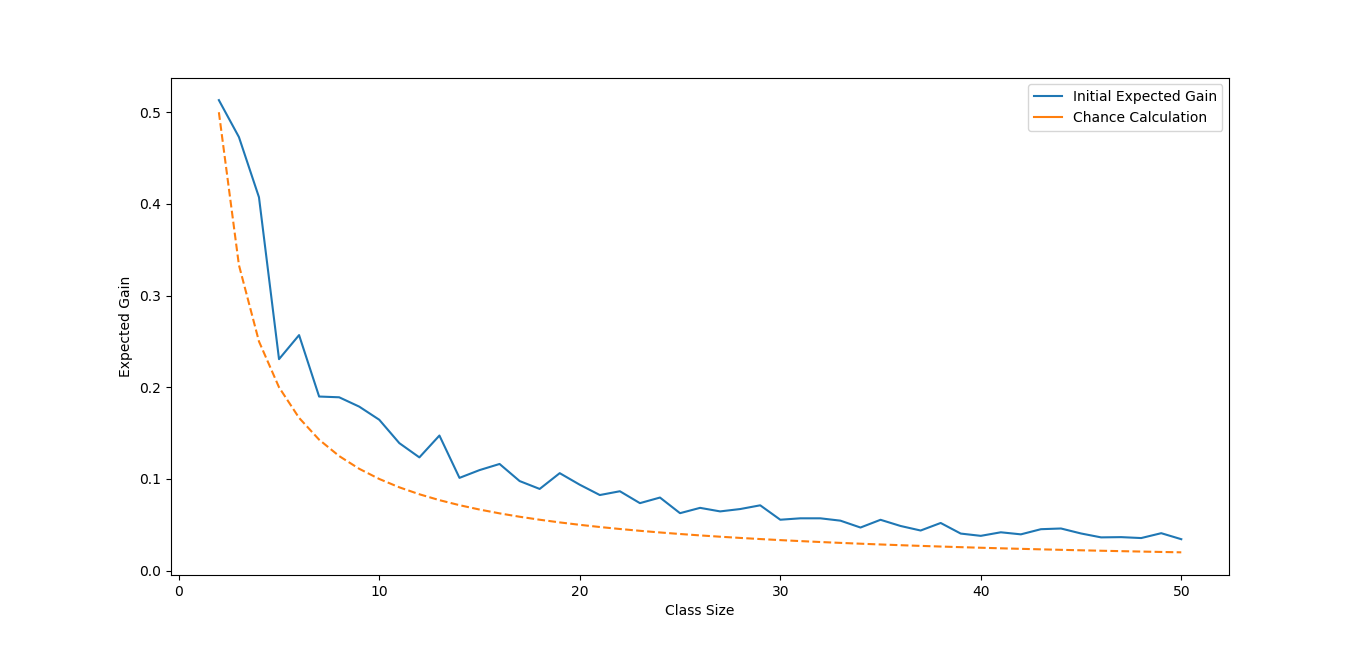
\includegraphics[scale=0.23]{iterativeClassInitialComparison.png}}
\caption{Effects of class size on initial Expected Gain, Comparison with Chance}
\label{fig}
\end{figure}
With this plot suggesting a general trend of the Bayesian classifier exceeding chance calculation prior to fitting, a Wilcoxon test was performed between the two distributions. Calculating a Wilcoxon statistic of 0, $p=1.1101*10^{-9}$,  the null hypothesis that these values come from the same distribution  was rejected, permitting an assertion that this above-chance performance is a trend of Bayesian classification. 

\subsection{Class and Sample Correlation}
Another trend can be observed with the increase in expected gain with sampling size for all classifiers excluding group $K=2$. Conversely, a decrease in fitted performance is observed in increasing complexity of classes. With sample sizes equal, the increase in $K$ appears proportional to a decrease in fitting accuracy. 

To better observe these trends, two sets of experiments were performed. The first was to observe initial and fitted performance over iterative increase in class complexity. A classifier was constructed on $100000$ randomized samples from the same measurement space as above. Initial and fitted expected gains were classified from $K=2$ to $K=50$, with $K$ increased by an 1 for each set of experiments. New seeds were provided for each variation of $K$ and a new delta of $.01$ was selected. Visualizations of both initial and fitted results are shown in [Figure 2] and [Figure 3]. 
\begin{figure}[htbp]
\centerline{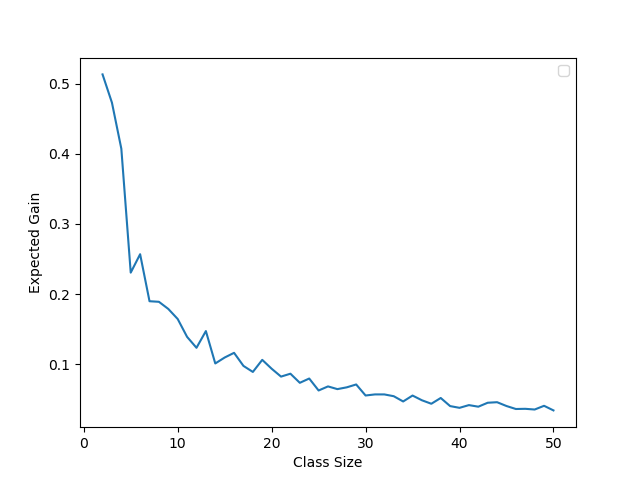
\includegraphics[scale=0.5]{iterativeClassInitial.png}}
\caption{Effects of class size on initial Expected Gain}
\label{fig}
\end{figure}
\begin{figure}[htbp]
\centerline{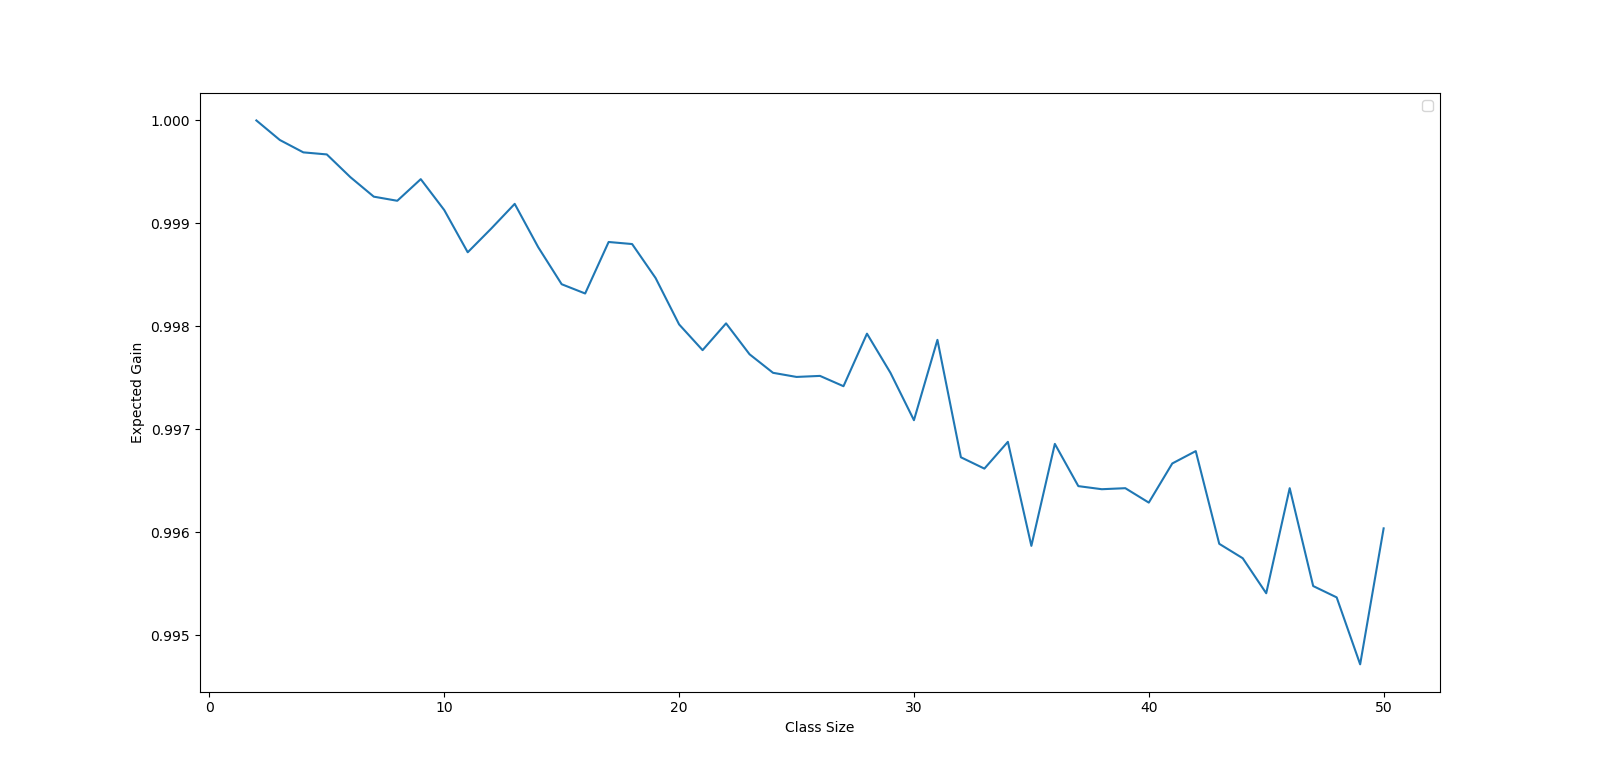
\includegraphics[scale=0.25]{iterativeClassFitted.png}}
\caption{Effects of class size on fitted Expected Gain}
\label{fig}
\end{figure}

With the data strongly suggesting a relationship between class size and expected gain for both initial and fitted data, correlation test were performed. As both may be assumed non-parametric distributions ($W_{initial}=41.9816$, $p_{initial}=7.6527 * 10^{-10}$, $W_{fitted}=5.93387$, $p_{fitted}=0.05146$), Spearman's coefficient was calculated for both: 

\begin{equation*}
\rho_{initial}=-0.98510, p_{initial}=1.3684 * 10^{-37}
\end{equation*}
\begin{equation*}
\rho_{fitted}=-0.98510, p_{fitted}=3.01079* 10^{-30}
\end{equation*}
Rejecting the null hypothesis of no correlation. 

The second series of experiments were conducted as above, save with variation of sample size. Holding $K=2$ (chosen for ease of calculation), classifiers were tested and fitted on sample sizes $Z=1000, ....,100000$, increasing by 1000 for each new classifier, with seeds randomized for each new classifier. A plot of expected gane over sample size for initial measures is presented in [Figure 4] and fitted values in [Figure 5].
\begin{figure}[htbp]
\centerline{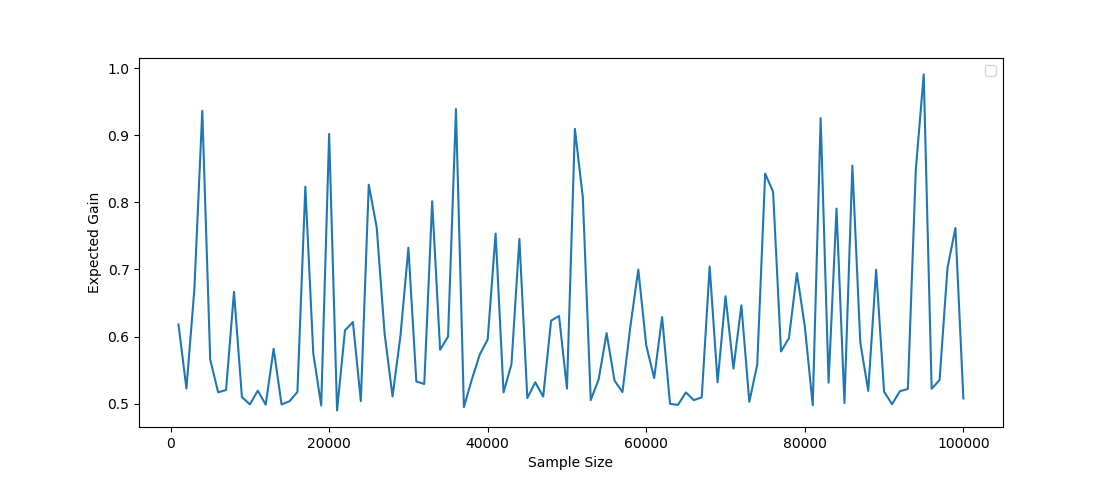
\includegraphics[scale=0.4]{iterativeSampleInitial.png}}
\caption{Effects of class size on initial Expected Gain}
\label{fig}
\end{figure}
\begin{figure}[htbp]
\centerline{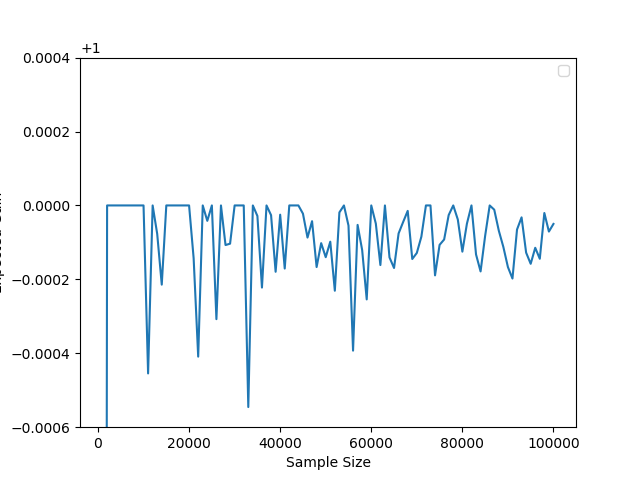
\includegraphics[scale=0.5]{iterativeSampleFitted.png}}
\caption{Effects of class size on fitted Expected Gain}
\label{fig}
\end{figure}

With a Shapiro test showing  the null-hypothesis of normal distribution ($p_{initial}=5.9600*10^{-5}$ and $p_{fitted}=5.7104*10^{-47}$), Spearman coefficients were calculated for both. The respective results were:
\begin{equation*}
\rho_{initial}=-0.08479, p_{initial}=0.4016
\end{equation*}
\begin{equation*}
\rho_{fitted}=-0.3005, p_{fitted}=0.0024
\end{equation*}
For the initial measures, we cannot reject the null-hypothesis of no correlation between sample size and expected gain. For fitted measures, we reject the null-hypothesis and note a slight negative correlation ($\geq-0.5$) for the fitted data.
\subsection{Fitting}
The increase in expected gain for each iteration of fitting is charted as below, with same proportions of Z charted together for comparison. 
\begin{figure}[htbp]
\centerline{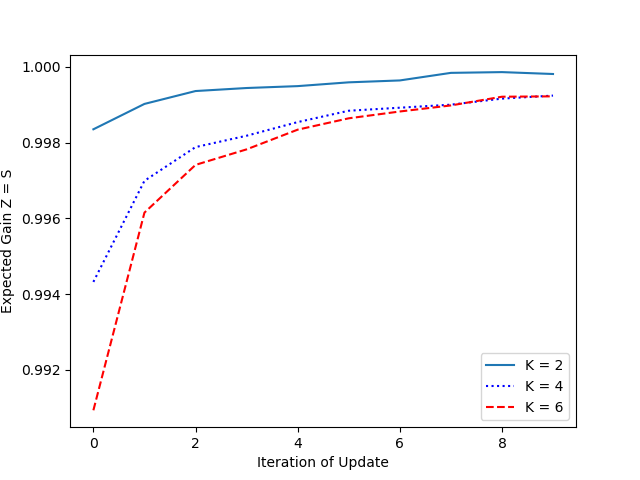
\includegraphics[scale=0.5]{Z_S.png}}
\caption{Iterative Improvements for Z=S}
\label{fig}
\end{figure}
\begin{figure}[htbp]
\centerline{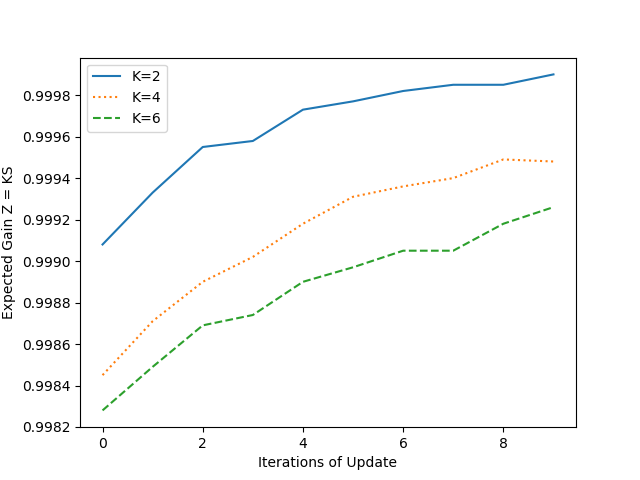
\includegraphics[scale=0.5]{Z_KS.png}}
\caption{Iterative Improvements for Z=KS}
\label{fig}
\end{figure}
\begin{figure}[htbp]
\centerline{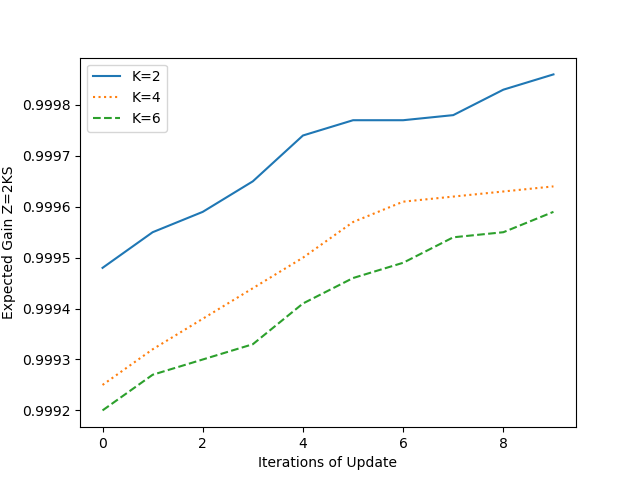
\includegraphics[scale=0.5]{Z_2KS.png}}
\caption{Iterative Improvements for Z=2KS}
\label{fig}
\end{figure}
The graphs visualize a few trends. Fitting has greater efficacy for less complex measurement spaces regardless of sample size, with $K=2$ having higher gain for all groups and $K=6$ having lowest gain. This supports the earlier trend noting the increase in class size being correlated with decrease in expected gain.

Also worth noting is the tendency of classifiers for $K=4$ and $K=6$ to maintain closer proximity to each other than those of $K=2$. This suggests that increasing class complexity and decreasing expected gain are not in a linear relationship and have a lower rate with each additional class. 
\section{Discussion and Conclusion}
\subsection{Discussion}
The baseline performance  for the classifiers provides a rather apt demonstration of the robustness of Bayesian classification. Despite likely erroneous conditional values $P(d|c)$, the estimation of class probability distributions provides the classifier enough stability to perform above chance. While this observation may be banal (obviously making classification decisions informed by likely distribution allows performance beyond chance), it deserves mention if only to reflect on how such features allow Bayesian classifiers to mitigate possible limitations regarding any poverty of class-conditional observations.

That classification over all fitted samples achieved near equal (within three significant digits) expected gains suggests the classifier has relatively little dependence on sample sizes given an idealized testing environment. From our experiment, the most significant case of measurement effect came only from fitted data (i.e. measurements that were biased toward altering performance). That this effect was only slight even for data that likely could not provide sufficient complexity to provide accurate training, lends credence to the observation that sample sizes have minimal effects on Bayesian classification. This seems to confirm the observations of Ng and Jorand in which Bayesian classifiers reach their asymptotic error at a quicker rate than other classifiers and thus require less training data in proportion to the number of parameters \cite{b3}.

The observation of strong negative correlation ($\leq-0.75$) between class size and performance is also worth noting. Notably in [Figure 2] is the appearance of logarithmic decrease among error size, suggesting a lower bound for error despite increasing complexity in size. That this error can be converted to a linear relationship with ideal data also assists in illustrating the robust nature of Bayesian classification: in disadvantagenous senarios there is a lower bound on poor performance and in advantageous scenarios it is less sensitive to data complexity. 
\subsection{Conclusion}
Bayesian classification is an incredibly robust methodology of predictive classification that can be generally invariant over training size and range of class values in an idealized environment. Though conceptually simple in comparison to other methodologies, this simplicity appears to be crucial in their performance and ability to mitigate even disadvantageous initialization environments. Provided idealized environments, they can perform at near perfect accuracy, providing an invaluable tool for machine learning applications.
\begin{thebibliography}{00}
\bibitem{b1}K. M. Al-Aidaroos, A. A. Bakar and Z. Othman, "Naïve bayes variants in classification learning," \textit{2010 International Conference on Information Retrieval and Knowledge Management (CAMP)}, Shah Alam, Selangor, 2010, pp. 276-281.
\bibitem{b2} D. Jurafsky and J. H. Martin, \textit{Speech and Language Processing: An Introduction to Natural Language Processing, Computational Lingusitics, and Speech Recognition}. 3rd ed., Draft. 2019.
\bibitem{b3} A. Y. Ng and M.I. Jordan. ``On Discriminative vs. Generative classifiers: A comparison of logistic regression and naive Bayes.'' \textit{Advances in Neural Information Processing Systems 14}, eds T.G. Dietterich, S. Becker, and Z. Ghahramani, pp. 841-848. MIT Press, 2002.
\bibitem{b4} A. Smola and S. V. N. Vishwanathan, \textit{Introduction to Machine Learning}. Cambridge, U.K: Cambridge University Press, 2008.
\end{thebibliography}
\end{document}
